% Chapter Chapter 4 For Reproducible Research in R and RStudio
% Christopher Gandrud
% Created: 16/07/2012 05:45:03 pm CEST
% Updated: 10 October 2012




\chapter{Getting Started with File Management}\label{DirectoriesChapter}

Careful file management is crucial for reproducible research. Remember two of the guidelines from Chapter \ref{GettingStartedRR}:

\begin{itemize}
    \item Reproducible research projects are many files explicitly tied together,
    \item Have a plan to organize, store, and make your files available. 
\end{itemize}

Apart from the fleeting situations where you have an email exchange (or even meet in person) with someone interested in reproducing your research, the main information independent researchers have about the procedures you used will be stored across many files: data files, analysis files, and presentation files. If these files are well organized and the links tying them together are clear, replication will be much easier. File management is also important for you as a researcher, because if your files are well organized you will be able to more easily make changes, collaborate with others, and so on. 

Using tools such as R, {\emph{knitr}, and markup languages like LaTeX requires fairly detailed knowledge of where files are stored--their {\bf{file path}}\index{file path}--in your computer. Handling files reproducibly also requires us to use command line tools to access and organize our files. R and Unix-like shell programs allow us to control files--creating, deleting, moving them--in powerful and really reproducible ways. By typing these commands we are documenting every step we take. This is a major advantage over graphical user interface type systems where we organize files by clicking and dragging them with the cursor. However, text commands require us to know our files' specific address--it's file path. 

In this chapter we discuss how a reproducible research project may be organized and cover the basics of file path naming conventions\index{file path naming conventions} in Unix, Mac, and Windows systems. We then learn organize them with RStudio Projects\index{RStudio Projects}. Finally, we will cover some basic R and Unix-like shell commands for manipulating files as well as how to navigate through files in RStudio in the {\bf{Files}} pane and. The skills we learn in this chapter will be heavily used in the next chapter (Chapter \ref{Storing}) and throughout the book.

In this chapter we work with locally stored files\index{locally stored}, i.e. files stored on your computer. In the next chapter we will discuss various ways to store and access files remotely in the cloud\index{cloud storage}.


\section{File paths \& naming conventions}

All of the operating systems\index{operating systems} covered in this book organize files in hierarchical directories\index{directories} (or file trees). To a large extent, `directories' can be thought of as the folders you usually see on your Windows or Mac desktop.\footnote{To simplify things, I use the terms `directory' and `folder' interchangeably in this book.} They are called `hierarchical' because directories are located inside of other directories, like we will see in Figure \ref{ExampleTree}. 

\subsection{Root directories}

A root directory\index{root directory} is the first level in a disk, such as a hard drive. It is the root out of which the file tree `grows'. All other directories are subdirectories\index{subdirectory} of the root directory.\footnote{On Windows computers you can have multiple root directories, one for each storage devise or partition of a storage device.}


On Windows computers the root directory is given a drive letter assignment\index{drive letter assignment}. If you use Windows regularly you will most likely be familiar with the \texttt{C:\textbackslash{}} used to denote the C partition of the the hardrive. This is a root directory. On Unix-like systems, including Mac computers. The root directory is simply labeled \texttt{/} with nothing before it.

\subsection{Subdirectories}

You will probably not store all of your files  the root directory. This would get very messy. Instead you will likely store your files in subdirectories of the root directory. Inside of these subdirectories may be further subdirectories and so on.  The directory a subdirectory is inside of is called the parent directory\index{parent directory}.

On Windows computers separate subdirectories are indicated with a back slash (\textbackslash{}). For example if we have a folder called {\emph{Data}} inside of a folder called {\emph{ExampleProject}} which is located in the C root directory it has the address \texttt{C:\textbackslash{}ExampleProject\textbackslash{}Data}.\footnote{For more information on Windows file path names see this helpful website: \url{http://msdn.microsoft.com/en-us/library/windows/desktop/aa365247(v=vs.85).aspx}} When you type Windows file paths into R you need to use two backslashes rather than one: \texttt{C:\textbackslash{}\textbackslash{}ExampleProject\textbackslash{}\textbackslash{}Data}. This is because the \texttt{\textbackslash{}} is an escape character\index{escape character} in R.\footnote{As we will see in Part IV, it is also a LaTeX escape character.} Escape characters tell the R to interpret the next character or sequence of characters differently. For example, on page \pageref{TSVEscape} you'll see how \texttt{\textbackslash{}t} can be interpreted by R as a tab. To neutralize the escape character simply add another escape character, i.e. escape the escape character. In R this simply means using a double backslash: \texttt{\textbackslash{}\textbackslash{}}. Another option for writing Windows file names is to use one forward slash (\texttt{/}).  

On Unix-like systems, including Mac computers, directories are indicated with a forward slash (\texttt{/}). The file path of the {\emph{Data}} file on a Unix-like system, for example: \texttt{/ExampleProject/Data}

In the book I switch between the two file system naming conventions to expose you to both.

\subsection{Working directories}

When you use R, the command line, and markup languages it is important to keep in mind what your current working directory is\index{working directory}. The working directory is the directory where the program automatically look for files and other directories. It is also where it will save files. Later in this chapter we will cover commands for handling the working directory.

\section{Organizing your research project}

Figure \ref{ExampleTree} gives an example of how the files in a simple reproducible research project could be organized. The project's main parent directory is called {\emph{Example Project}}. Inside this directory are three subdirectories: a data gathering directory, an analysis directory, and a presentation directory. Each of these directories contain further subdirectories and files. The {\emph{Presentation}} directory for example contains subdirectories for files that present the findings in article, slideshow, and website formats.

\clearpage
\thispagestyle{plain}
\begin{landscape}
\begin{figure}[th!]
    \caption{Example Research Project File Tree}
    \label{ExampleTree}
    \begin{center}
    
    \documentclass{article}

\usepackage{tikz}

\begin{document}

%%%%%% Example 

\tikzstyle{DirBox} = [draw=black, rectangle, minimum width=5em, thick]
  
\begin{tikzpicture}
  % Root Directory
  \node (root) at (5, 10) [DirBox]{Root};
  
  % Project Directory
  \node (project) at (5, 8.5) [DirBox]{Project};
  
  % Main Project sub-directories
  \node (data) at (2, 7) [DirBox]{Data};
  \node (analysis) at (5, 7) [DirBox]{Analysis};
  \node (presentation) at (8, 7) [DirBox]{Presentation};
  
  % Data subdirectories/files
  \node (dataGatherSource) at (-0.5, 6) [DirBox]{GatherSource};  
  \node (dataFiles) at (2, 6) [DirBox]{DataFiles};
  
  \node (dataMake) at (-0.5, 5.25) {{\small{DataMakeFile.R}}};
  
  \node(dataGather) at (-0.5, 4.5) [DirBox]{IndvDataGather};
  \node (dataGather1) at (-0.5, 3.5) {{\small{DataGather1.R}}};
  
  % Analysis subdirectores/files
  
  % Presentation subdirectories/files
  
  % Connect boxes
  \draw (root) -- (project);
  \draw (project) -| (data);
  \draw (project) -- (analysis);
  \draw (project) -| (presentation);
  
  %% Data connect boxes
  \draw (data) -| (dataGatherSource);
  \draw (data) -- (dataFiles);
  \draw (dataGatherSource) -- (dataMake);
  
\end{tikzpicture}



\end{document}
    \end{center}
\end{figure}
\end{landscape}

In addition to this main folders you will probably notice a file called {\emph{README.md}} The {\emph{README.md}} file\index{README file} gives an overview of all the files in the project. It should briefly describe the project including things such as its title, author(s), topic and so on. It should also indicate how the folders in the project are organized and give instruction for how to reproduce the project. The README file should be in the main project folder--in our example this is called {\emph{ExampleProject}}--so that it is easy to find. If you are storing your project as a GitHub\index{GitHub} repository (see Chapter \ref{Storing}) and the file is called \texttt{README} its contents will automatically be displayed on the repository's main page. If it is written using Markdown, it will also be properly formatted.

It is good practice to dynamically include the system information for the R session you used to create the project. To do this you can write your readme file with R Markdown (see Chapter \ref{LargeDocs}). Simply include the \texttt{sessionInfo()} command in a code chunk in the R Markdown document. If you knit this file immediately after knitting your presentation document it will record the information for that session.

\noindent You can also dynamically include session info in a LaTeX document. To do this simply use the {\tt{toLatex}} command in a code chunk. The code chunk should have the option \texttt{results='asis'}. The code is:

\begin{knitrout}
\definecolor{shadecolor}{rgb}{0.969, 0.969, 0.969}\color{fgcolor}\begin{kframe}
\begin{alltt}
\hlfunctioncall{toLatex}(\hlfunctioncall{sessionInfo}())
\end{alltt}
\end{kframe}
\end{knitrout}


%% Make file discussion?

\section{RStudio Projects}

If you are using RStudio, you may want to organize your files as Projects\index{RStudio Projects}. You can declare that a directory should be a Project by clicking on \texttt{Project} in the RStudio menu bar and selecting \texttt{Create Project\ldots}. A new window will pop up. Select the option \texttt{Existing Directory}. Find the directory you want to make an RStudio Project by clicking on the \texttt{Browse} button. Finally, select \texttt{Create Project}. You will also notice in the Create Project pop up window that you can create projects in new directories and also create a project from a directory already under version control (we'll do this in Chapter \ref{Storing}). When you create a new project you will see that a file with the extension \texttt{.Rproj} is created in the directory.

Making your research project directories RStudio Projects is useful in a number of ways:

\begin{itemize}
    \item when you open the \textttt{.Rproj} file RStudio automatically sets the working directory to the Project's directory and loads the project workspace, history, and source code files you were last working on.
    \item you can set project specific options like what whether or not your PDF presentation documents should be compiled with Sweave or {\emph{knitr}}.
    \item when you close the project your R workspace and history are saved in the project directory,
    \item gives you a way to version control your files.
\end{itemize}

%%%%%%%%%%%%%%% File Manipulation
\section{R file manipulation commands}

R has an a powerful set of commands for handling and navigating through files. Including these commands in our source code files allows us to more easily replicate our actions.

\paragraph{{\tt{getwd}}}\index{getwd}

To find out what current working directory R is using type:

\begin{knitrout}
\definecolor{shadecolor}{rgb}{0.969, 0.969, 0.969}\color{fgcolor}\begin{kframe}
\begin{alltt}
\hlfunctioncall{getwd}()
\end{alltt}
\begin{verbatim}
## [1] "/git_repositories/Rep-Res-Book/Source/Children/Chapter4"
\end{verbatim}
\end{kframe}
\end{knitrout}


\noindent The example here shows you the current working directory that was used while knitting this chapter.

\paragraph{{\tt{list.files}}}\index{list.files}

Use the \texttt{list.files} command see all of the files and subdirectories in the current working directory. You can list the files in other directories too by adding the directory path as an argument to the command.  

\paragraph{{\tt{setwd}}}\index{setwd}

The {\tt{setwd}} command sets the current working directory\index{working directory}. For example, if we are on a Mac or other Unix-like computer we can set the working directory to the {\emph{GatherSource}} directory in our Example Project (see Table \ref{ExampleTree}) like this

\begin{knitrout}
\definecolor{shadecolor}{rgb}{0.969, 0.969, 0.969}\color{fgcolor}\begin{kframe}
\begin{alltt}
\hlfunctioncall{setwd}(\hlstring{"/ExampleProject/Data/GatherSource"})
\end{alltt}
\end{kframe}
\end{knitrout}


\noindent Now R will automatically look in the {\emph{GatherSource}} folder for files and will save new files into this folder, unless we explicitly tell it to do otherwise.

\paragraph{{\tt{dir.create}}}\index{dir.create}

Sometimes we may want to create a new directory. We can use the {\tt{dir.create}} command to do this.\footnote{Note: you will need the correct system permissions to be able to do this.} For example to create a {\emph{ExampleProject}} file in the root C directory on a Windows computer type:

\begin{knitrout}
\definecolor{shadecolor}{rgb}{0.969, 0.969, 0.969}\color{fgcolor}\begin{kframe}
\begin{alltt}
\hlfunctioncall{dir.create}(\hlstring{"C:\textbackslash{}\textbackslash{}ExampleProject"})
\end{alltt}
\end{kframe}
\end{knitrout}


\paragraph{{\tt{file.create}}}\index{file.create}

Similarly, you can create a new blank file with the \texttt{file.create} command. To add a blank R source code file called {\emph{SourceCode.R}} to the {\emph{ExampleProject}} directory on the C drive use:

\begin{knitrout}
\definecolor{shadecolor}{rgb}{0.969, 0.969, 0.969}\color{fgcolor}\begin{kframe}
\begin{alltt}
\hlfunctioncall{file.create}(\hlstring{"C:\textbackslash{}\textbackslash{}ExampleProject\textbackslash{}\textbackslash{}SourceCode.R"})
\end{alltt}
\end{kframe}
\end{knitrout}


\paragraph{{\tt{unlink}}}\index{unlink}

Finally, you can use the {\tt{unlink}} command to delete a file, files, or directories. 

\section{Unix-like shell commands for file management} 

Though this book is mostly focused on using R for reproducible research it can be useful to use a Unix-like shell program to manipulate files in large projects. A command line shell program is simply a program that allows you to type commands to interact with your computer's operating system. We will especially return to shell commands near the end of the book when we discuss make files\index{make file} for compiling large documents, and batch reports\index{batch reports} (Chapter \ref{LargeDocs}). The syntax discussed here is also similar to the used in command line git (Chapter \ref{Storing}) and Pandoc (Chapter \ref{LargeDocs}). We don't have enough space to properly get started with shell programs. For good introductions for Unix and Mac OS 10 computers see William E. Shotts Jr.'s book on the Linux command-line\cite[]{ShottsJr2012}. For Windows users, Microsoft maintains a tutorial on Windows PowerShell at \url{http://technet.microsoft.com/en-us/library/hh848793}.

The one piece of general instruction I will give now is to highlight an important difference in the syntax between R and shell commands. In shell commands you don't need to put parentheses around your arguments. For example if we want to change our working directory to my Mac Desktop in a shell using the {\tt{cd}} command we simply type:

\begin{knitrout}
\definecolor{shadecolor}{rgb}{0.969, 0.969, 0.969}\color{fgcolor}\begin{kframe}
\begin{verbatim}
cd /Users/Me/Desktop
\end{verbatim}
\end{kframe}
\end{knitrout}


\todo[inline]{The remainder of this chapter is incomplete.}

\paragraph{{\tt{cd}}}\index{cd}

As we just saw, to change the working directory in the shell can just use the {\tt{cd}} (change directory) command.

\paragraph{{\tt{rm}}}

The {\tt{rm}}\index{rm} command is similar to R's {\tt{unlink}} command. It deletes files or directories.

R also has an \texttt{rm} command. It is different because it removes objects from your R workspace rather than files from your working directory.

\section{File navigation in RStudio}

The RStudio {\bf{Files}} pane allows us to navigate and do some basic file manipulation. Figure \ref{FilesPane} shows us what this pane looks like.

\begin{figure}[t!]
    \caption{The RStudio Files Pane} %\\[0.25cm]
    \label{FilesPane}
        \begin{center}    
        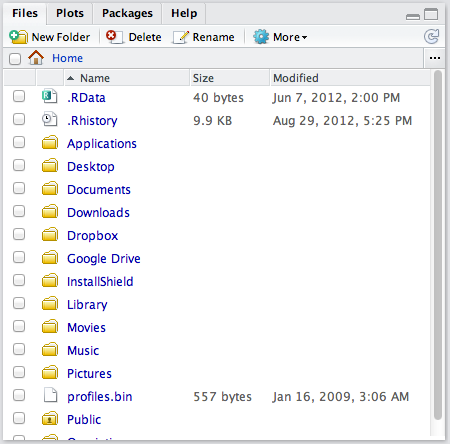
\includegraphics[scale=0.4]{/git_repositories/Rep-Res-Book/Source/Children/Chapter4/images4/RStudioFiles.png}
        \end{center}
\end{figure}
